\documentclass[fleqn]{beamer}

\usetheme[
  progressbar=frametitle,    % or try: 'none', 'foot'
  numbering=fraction,        % frame number / total
  sectionpage=none,
  subsectionpage=none
]{metropolis}

\title{Week 4 \\ Part B \\ Tools for Understanding}
\author{Hans Halvorson}
\date{May 19, 2025}

% Load math packages
\usepackage{amsmath,amssymb}

% Highlighting commands
\usepackage{soul}

% Optional: custom keyword formatting
\newcommand{\kw}[1]{\textbf{#1}}

% Only show section numbers in TOC
\setbeamertemplate{section in toc}[sections numbered]

% Section title slide at each new section
\AtBeginSection[]
{
  \begin{frame}
    \frametitle{Table of Contents}
    \tableofcontents[currentsection]
  \end{frame}
}

% Minimalist footer and navigation
\setbeamertemplate{footline}[frame number]
\setbeamertemplate{navigation symbols}{}

% Ensure numbered sections (useful with TOC)
\setcounter{secnumdepth}{1}

\begin{document}



\begin{frame}
  \titlepage
\end{frame}

\begin{frame}{Table of Contents}
\tableofcontents
\end{frame}

\section{A pluralist account of understanding}


\begin{frame}

  \begin{itemize}
  \item De Regt and Dieks: Understanding cannot be reduced to any of
    these particular accounts of scientific explanation
  \item HH: De Regt and Dieks do \emph{not} say that understanding
    requires at least one of these types of explanations. This seems
    like a defect of permissiveness in their account.
  \end{itemize}

\end{frame}  

\subsection{Causation not required for understanding}
  
\begin{frame}

\begin{itemize}
\item ``Salmon treats causality as a standard for intelligibility'' (p
  144)
\item ``Present-day scientific developments cast severe doubt on the
  alleged privileged status of [Salmon's] model of causal explanation
  as the way to scientific understanding.'' (p 145)
\item ``At the deepest levels of physical reality Salmon's concept of
  causality is highly problematic.'' (p 145)
\item ``Physics is full of examples that show that causal-mechanical
  explanation is not always the actually preferred manner of achieving
  understanding.'' (p 145)
\end{itemize}
  
\end{frame}


\begin{frame}{Quantum mechanics}

  \begin{itemize}
  \item ``Causal connections of this type \dots do not exist according
    to quantum theory in its standard interpretation.'' (p 145)
    \begin{itemize}
    \item Arguments against trajectories
    \item Bell non-locality
    \end{itemize}
  \end{itemize}
\end{frame}

\begin{frame}{Lorentz contraction}

  \begin{itemize}
  \item ``The usual way of making the contractions intelligible is by
    connecting them deductively to the basic posulates of special
    relativity (the relativity postulate and the light
    posulate). \dots Causal reasoning is not involved.''  (p 146)
  \item More controversial than De Regt and Dieks make it out to
    be. See Bell, ``How to teach special relativity'' or H. Brown,
    \emph{Physical Relativity} \end{itemize} 

\end{frame}

\begin{frame}{Deflection of light by matter in GTR}

  ``The just-mentioned example undermines the causal conception of
  understanding, because no causal chains were identified that are
  responsible for the deflection of the light.'' (p 157)

\end{frame}

\begin{frame}

  \begin{itemize}
  \item ``But even in pre-twentieth-century physics causal-mechanical
    explanation was not always the norm.'' (p 146)
  \item ``Between 1700 and 1850 action-at-a-distance rather than
    contact action and causal chains dominated the scientific scene.''
    (p 146)
  \end{itemize}

\end{frame}

\begin{frame}

  \begin{itemize}
  \item ``These facts are sufficient to cast doubt on the core idea
    that causality has a special status as \emph{the} fundamental,
    privileged standard of intelligibility.'' (p 146)
  \item ``It would be erroneous to maintain that visualization is
    essential for obtaining understanding.'' (p 156)
  \item ``The various intelligibility standards proposed by
    philosophers of science (e.g., visualizability, causality, and
    continuity) find a place in our approach as `tools' for achieving
    understanding: they can help to `see intuitively' the consequences
    of a scientific theory.'' (p 157)
  \end{itemize}

\end{frame}

\begin{frame}{Does causality have a privileged role?}

  \begin{itemize}
  \item ``By the guidance which analysis in terms of cause and effect
    has offered in many fields of human knowledge, the principle of
    causality has even come to stand as the ideal for scientific
    explanation.'' (Bohr 1948)
  \item ``The viewpoint of complementarity presents itself as a
    rational generalization of the very ideal of causality.'' (Bohr
    1948)
  \end{itemize}
  
\end{frame}


\subsection{Unification not required for understanding}

\begin{frame}

  \begin{itemize}
  \item ``Unification appears to be an effective tool for achieving
    understanding, but like causality it is one among a variety of
    tools.'' (p 149)
  \item ``The various intelligibility standards proposed by
    philosophers of science (e.g., visualizability, causality, and
    continuity) find a place in our approach as `tools' for achieiving
    understanding.'' (p 156--157)
  \end{itemize}

\end{frame}

\section{Understanding according to De Regt and Dieks}

\begin{frame}{Criterion for Understanding Phenomena}

  \textbf{CUP:} A phenomenon $P$ can be \textbf{understood} if a
  theory $T$ of $P$ exists that is intelligible.

\end{frame}

\begin{frame}{Criterion for the Intelligibility of Theories}
  
  \textbf{CIT:} A scientific theory $T$ is \textbf{intelligible} for
  scientists (in context $C$) if they can recognize qualitatively
  characteristic consequences of $T$ without performing exact
  calculations.


  \vspace{2em} ``What one wants in science is the ability to grasp how
  the predictions are brought about by the theory.'' (p 151)
  
\end{frame}

\begin{frame}[allowframebreaks]{Understanding Boyle’s Law via the Kinetic Theory}

\small
\textbf{Illustration of CUP and CIT:} How the kinetic theory provides understanding of gas behavior.

\vspace{0.5em}
\begin{itemize}
  \item \textbf{Qualitative model:} Boltzmann’s kinetic theory pictures a gas as a collection of freely moving molecules.
  \item \textbf{Temperature =} average kinetic energy of molecules.
  \item \textbf{Pressure =} cumulative force from molecular collisions with the container walls.
\end{itemize}

\vspace{1em}
\begin{center}
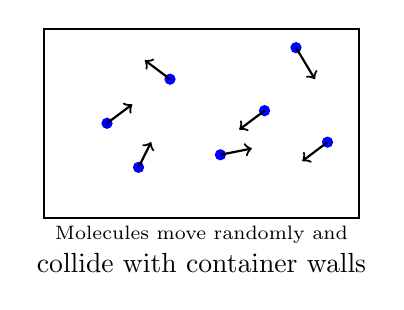
\begin{tikzpicture}[scale=0.8]
  % Container
  \draw[thick] (0,0) rectangle (5,3);

  % Molecules
  \foreach \x/\y in {1/1.5, 2/2.2, 3.5/1.7, 4/2.7, 1.5/0.8, 2.8/1, 4.5/1.2} {
    \filldraw[blue] (\x,\y) circle (0.08);
  }

  % Velocity arrows
  \draw[->,thick] (1,1.5) -- (1.4,1.8);
  \draw[->,thick] (2,2.2) -- (1.6,2.5);
  \draw[->,thick] (3.5,1.7) -- (3.1,1.4);
  \draw[->,thick] (4,2.7) -- (4.3,2.2);
  \draw[->,thick] (1.5,0.8) -- (1.7,1.2);
  \draw[->,thick] (2.8,1) -- (3.3,1.1);
  \draw[->,thick] (4.5,1.2) -- (4.1,0.9);

  % Label
  \node[align=center] at (2.5,-0.5) {\scriptsize Molecules move randomly and\\collide with container walls};

\end{tikzpicture}
\end{center}

\framebreak

\small
\textbf{Key insights (no equations):}
\begin{itemize}
  \item Adding heat $\Rightarrow$ molecules move faster $\Rightarrow$ more forceful, frequent collisions $\Rightarrow$ higher pressure.
  \item Reducing volume $\Rightarrow$ more collisions per unit area $\Rightarrow$ higher pressure (at constant temperature).
\end{itemize}

\vspace{0.5em}
\textbf{Conclusion:} The kinetic theory provides an intelligible, causal-mechanical picture that explains Boyle’s law qualitatively — in line with CUP and CIT.

\end{frame}



\begin{frame}{Problems with CIT?}

  \begin{itemize}
  \item CIT is ambiguous. Imagine a mechanical arm that pulls slips of
    paper out of a barrel, and always pulls out correct
    predictions. Would we be satisfied knowing how the mechanical arm
    operates?
  \item It seems that we would want to know how the mechanical arm
    manages to get the predictions right. We would want an explanation
    not of how it generates predictions, but of why it generates the
    right predictions 
    \end{itemize}



\end{frame}


\begin{frame}{Open questions}


  \begin{itemize}
  \item Does the account of De Regt and Dieks have any normative
    content? Or does it just point out the fairly obvious fact that
    scientific sub-communities have ideals for understanding?
  \item They point out that the Copenhagen-G{\"o}ttingen physicists
    found matrix mechanics to be intelligible, while most other
    physicists disagreed. (p 141)
  \end{itemize}



\end{frame}



\section{Tools for understanding}

\begin{frame}

  \begin{itemize}
  \item So far we have been talking about the abstract theory of
    scientific understanding --- i.e.\ what, in theory, is
    ``understanding'', and the claim (of de Regt and Dieks) that
    understanding is a primary goal of science
  \item We now turn to talking about (a) the role of \textbf{tools} in
    understanding, and (b) with specific reference to machine learning
    and AI
  \end{itemize}


\end{frame}

\begin{frame}{Tools for increasing scientific understanding}

\begin{columns}[T] \begin{column}{0.45\textwidth}

\begin{itemize}
    \item Writing!   
    \item Diagrams
    \item Illustrations 
    \item Scientific instruments
      \begin{itemize}
      \item Microscope
      \item Telescope
      \item Thermometer
      \item Barometer
      \end{itemize}
    \item Physical models
    \item Simulations 
    \end{itemize} \end{column}

  \begin{column}{0.45\textwidth} \includegraphics[scale=0.72]{hauch}
    \\ {\small source: Hauchs physiske cabinet} \end{column}

\end{columns}


\end{frame}

\begin{frame}{Why should (future) scientists think about AI?}

  \begin{itemize}
  \item Corporations such as OpenAI, Microsoft, and Google claim that
    AI will lead to new knowledge --- and not simply by eliminating
    tedious and repetitive tasks
  \item Will AI take your jobs? 
  \end{itemize}
  
  \end{frame}

\section{Three dimensions of computer-assisted scientific
  understanding}

\begin{frame}{Michie's classification of machine learning}

  \begin{description}
  \item[Weak ML:] improved prediction quality with larger amounts of
    training data (algorithm is treated as a black box)
  \item[Strong ML:] provides a symbolic representation of its
    hypothesis
  \item[Ultrastrong ML:] the algorithm teaches the human operator such
    that the human performance is improved compared with the human
    learning from the data alone
  \end{description}
\end{frame}

\begin{frame}

  When we talk about ML or AI helping science, what exactly is it that
  we are talking about?

  \begin{description}
  \item[Neural network] A computer system modelled on the human brain
    and nervous system
    \url{https://www.ibm.com/topics/neural-networks}
  \item[Deep learning] ``Deep learning is a subset of machine learning
    that uses multi-layered neural networks, called deep neural
    networks, to simulate the complex decision-making power of the
    human brain.''  (From the IBM website)
  \end{description}


\end{frame}

\begin{frame}{Dimension 1: Computational microscope}

  AI might be able to ``see'' things that are invisible to the ``naked
  eye''

    \begin{itemize}
    \item ``AI can act as an instrument revealing properties of a
      physical system that are otherwise difficult or even impossible
      to probe'' (p 761)
    \item ``[AI] can provide information not (yet) attainable through
      experimental means'' (p 763)
    \item ``\dots computational microscopes enable the investigation
      of objects or processes that cannot be visualized or probed in
      any other way, for example, biological, chemical or physical
      processes that happen at length and time scales not accessible
      in experiments.'' (p 764)
    \end{itemize}


\end{frame}

\begin{frame}

  \begin{itemize}
  \item What kinds of things can be seen, and how is AI supposed to do
    this?
    \begin{itemize}
    \item ``\dots the new computer-generated data''
    \item ``\dots new ways to analyze these systems without the need
      to perform full computations''
    \item ``\dots without the need for simulating the entire system''
    \end{itemize}
  \end{itemize}

\end{frame}



\begin{frame}

    ``Not only is training a neural network much faster and
    computationally less expensive than running a hydrodynamical
    simulation, it also does not rely on strong assumptions about the
    underlying physics, or suffer from limitations arising from coarse
    resolution.'' (Schawinski et al. 2018, p 3)

\end{frame}


\begin{frame}{Improvements of computational microscopes?}

  \begin{enumerate}
  \item Increasingly complex systems: size, timescale, number of
    interactions
  \item Advances in data representation
  \end{enumerate}

\end{frame}

\begin{frame}{Dimension 2: Resource of inspiration}


  \begin{itemize}
  \item Throughout human history, people have tried to find a recipe
    for inspiration
  \item Much scientific innovation seems to happen by luck, or even as
    if by magic
  \item In many cases, macro-level circumstances produced ideal
    conditions for innovation
    \begin{itemize}
    \item E.g. Vienna circa 1900
    \end{itemize}
  \item Social privilege and freedom from other worries
    \begin{itemize}
    \item E.g. Niels Bohr's childhood (see Favrhold,
      \textit{Filosoffen Niels Bohr})
    \end{itemize}
  \end{itemize}

\end{frame}


\begin{frame}

\begin{enumerate}
\item[1.] Identifying surprises in data \newline ``Data anomalies can
  manifest themselves in a more involved combination of variables,
  which might be very difficult for humans to grasp.'' (p 764)
  \newline \textbf{autonomous anomaly detection} \end{enumerate}
\end{frame}

\begin{frame}
  \begin{enumerate}
    \item[2.] Identifying surprises in the scientific literature \newline
  ``Researchers have to specialize in narrow subdisciplines, which
  makes finding new interdisciplinary ideas difficult.'' (p 765)
  \begin{enumerate}
    \item[a.] Unsupervised word embedding of a large corpus of scientific
      papers
    \item[b.] Semantic networks built on large bodies of scientific
      literature
  \end{enumerate}
\end{enumerate}

\end{frame}

\begin{frame}
  \begin{enumerate}
  \item[3.] Surprising concepts by inspecting models \newline ``\dots
    rationalizing what AI algorithms have learned in order to solve a
    specific problem'' \newline ``\dots understand the model's
    internal worldview''
\end{enumerate}


\end{frame}

\begin{frame}

  ``The concepts rediscovered in all of those works were not new and,
  thus, the most important challenge for the future is to learn how to
  extract previously unkown concepts.'' (p 766)


\end{frame}

\begin{frame}

  \begin{enumerate}
  \item[4.] New concepts from interpretable solutions
  \end{enumerate}

\end{frame}

\begin{frame}

  \begin{enumerate}
  \item[5.] Probing the behavior of artificial agents
  \end{enumerate}

\end{frame}

\begin{frame}

    \begin{itemize}
    \item ``\dots an artificial muse, expanding the scope of human
      imagination and creativity''
    \item Can an AI inspire in a more directed way than, say, a walk
      in the forest?
    \end{itemize}
  
\end{frame}



\begin{frame}{Dimension 3: AI as an agent of understanding}

  \begin{itemize}
  \item ``Algorithms that can autonomously acquire new scientific
    understanding, and ultimately explain these insights to humans.''
    (p 766)
  \item An extreme scenario is that AIs become our peers or even our
    superiors as scientists.
  \item Granted, such a possibility is in the realm of
    speculation. However, what could this possibility actually look
    like?
  \item It seems that the best model we have at present is the
    teacher-student (or parent-child) relationship
  \item ``Both require that the machine gets new insights and teaches
    them to the human.'' (p 766)
  \end{itemize}


\end{frame}

\begin{frame}{Additional resources}

  {\small

    \begin{itemize}
    \item N. Bohr. ``On the notions of causality and complementarity''
      \textit{Dialectica}
    \item J. Faye. ``Niels Bohr’s experimentalist approach to
      understanding quantum mechanics''
    \end{itemize}

  }


\end{frame}



\end{document}
%%% Local Variables:
%%% mode: latex
%%% TeX-master: t
%%% End:
